\section{Introduction}
Robotic manipulation in the open world could greatly benefit from visual world models that predict how the environment would evolve given an agent’s interactions~\citep{zhao2026towards,zhao2025smap,li2026causal,agarwal2025cosmos,ali2025world}. 
While recent generative video models~\citep{ha2018recurrent,xiang2024pandora,zheng2024open,wang2025wan} have shown encouraging progress in policy synthesis~\citep{du2023learning,liang2024dreamitate,zhen2025learning}, data simulation and generation~\citep{zhu2024irasim}, and long-horizon planning~\citep{du2023video,li2025novaflow}, they remain limited by the 2D projective nature of pixels. This inherent limitation leads to a loss of critical spatial relationships, preventing precise 6-DoF pose estimation and depth-aware interaction~\citep{hu2024video,agarwal2025cosmos,li2026causal}. Furthermore, 2D models often lack geometric grounding,  leading to temporal inconsistencies such as fluctuating object scales and unphysical shape morphing, which hinders their utility in robust policy learning. Consequently, transitioning generative world modeling from 2D videos to geometry-integrated 4D scene evolution is an essential step toward a solid foundation for embodied intelligence.

Existing 4D scene-modeling approaches fall into two categories. The first builds on Neural Radiance Fields (NeRF)~\citep{mildenhall2021nerf} or 3D Gaussian Splatting (3DGS)~\citep{kerbl20233d}, which can be further divided into optimization-based methods~\citep{zhao2024sg,zhao2024hfgs,yu20244real,bahmani20244d} that are computationally intensive and scene-specific, and feed-forward models~\citep{ren2024l4gm,wu2025cat4d} that prioritize speed but typically focus on object-centric generation. These approaches often require multi-view inputs or struggle to scale to complex scene-level environments. The second category comprises dynamic Structure-from-Motion (SfM) approaches~\citep{wang2025continuous,li2025megasam}, which reconstruct time-varying point clouds but lack the generative capability to predict future states from a single image. Neither category readily provides a compact, scalable representation that integrates with the strong generative priors of pretrained video diffusion models.

\begin{figure}[t]
  \centering
    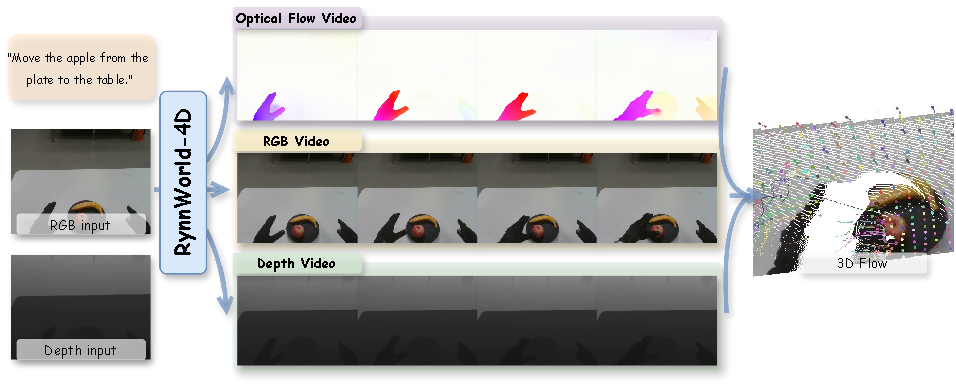
\includegraphics[width=\linewidth]{Fig/teasor.pdf}\\
  \caption{Given an input RGB-D image and description, \our generates RGB, depth, and optical flow videos synchronously, which can be further lifted into 3D scene flow (right).}
  \label{fig:teasor}
\end{figure}

To bridge this gap, we propose a lightweight projective 4D representation by predicting synchronized sequences of RGB, depth, and optical flow (RGB-DF): depth lifts each pixel to a 3D location, and depth together with optical flow can be back-projected into 3D scene flow under standard pinhole-camera assumptions, providing a per-point 3D motion cue (illustrated as the ``3D Flow'' in Fig.~\ref{fig:teasor}).
Compared to RGB-only sequences, this representation makes geometry and motion explicit; compared to explicit 3D volumes or 4D Gaussians, it stays in a 2D-aligned format and therefore inherits the scalability and the rich generative priors of large-scale video diffusion models.


Building on this representation, we present \textbf{\our}, a 4D embodied world model that, conditioned on a single RGB-D image and a text instruction, synchronously generates RGB, depth, and optical-flow videos within one shared denoising loop (Fig.~\ref{fig:teasor}).
Specifically, we extend a pretrained video diffusion model~\citep{wang2025wan} into a tri-branch transformer, where each branch handles one modality with independent transformer with shared cross attention keys/values across modalities, while Joint Cross-Modal Attention modules enforce cross-modal consistency.
This design preserves the strong generative priors of the pretrained backbone while allowing each modality to specialize, \textit{i.e.}, textures for RGB, spatial geometry for depth, and motion displacements for optical flow.
A key challenge for training \our is the absence of large-scale datasets with dense 4D annotations. To address this, we curate \textbf{Rynn4DDataset 1.0}, a large-scale hybrid dataset comprising over 254 million video frames drawn from egocentric human activity datasets~\citep{damen2020epic,wang2024egovid} and robotic manipulation datasets~\citep{wu2024robomind,liu2024rdt,jiang2025galaxea,wu2025robocoin,bu2025agibot}, each enriched with high-quality pseudo-annotations for depth and optical flow.


The RGB-DF representation offers a critical advantage: it aligns more closely with a robot’s action space than raw 2D pixel changes. Consequently, a downstream policy trained on \our's internal 4D representations bypasses the heavy structural inference typically required when operating on 2D latents alone. Leveraging this synergy, we introduce \textbf{\our-Policy}, an inverse dynamics head that extracts robot actions directly from \our’s predictive 4D features. By utilizing these internal latents in a single forward pass and bypassing the iterative denoising bottleneck, \our-Policy enables high-frequency, closed-loop control suitable for real-time interaction. In summary, our work makes the following contributions:

\begin{itemize}[labelsep=0.6em, leftmargin=1.2em,itemindent=0em]
\item We introduce a \textbf{projective 4D representation} that co-generates RGB, depth, and optical flow, and we show how it admits a natural 3D-scene-flow reading that makes geometry and motion explicit while staying compatible with large-scale video diffusion priors.
\item We develop \textbf{\our}, a tri-branch 4D world model that co-generates physically coherent RGB-DF sequences through mutual cross-modal interactions.
\item We curate \textbf{Rynn4DDataset 1.0}, a large-scale 4D embodied video dataset with depth and optical flow annotations for training 4D embodied world model.
\item We propose \textbf{\our-Policy}, which leverages the internal 4D representations to enable high-frequency, closed-loop robotic control. 
\end{itemize}

